\documentclass[12pt]{article}

\usepackage{sbc-template}

\usepackage{graphicx,url}

\usepackage[brazil]{babel}
\usepackage[utf8]{inputenc}
\usepackage{booktabs}


\sloppy

%\title{Integração de IA Generativa e Processamento de Áudio no Apoio à Alfabetização: A Proposta do Sistema que transforma leitura em desenvolvimento}

\title{Transformando Leitura em Desenvolvimento: O Uso de IA Generativa e Processamento de Áudio na Alfabetização}


%\author{Frederico H. Rocha\ins{1}, Caio C. Miranda\inst{2}, Jaime Silva\inst{2}, João P. B. Tomé\inst{2}, Jacson R. Barbosa\inst{1}, \\Valdemar V. Neto\inst{1} }


% \address{Instituto de Informática -- Universidade Federal de Goiás (UFG)
%    \email\{caio\_miranda, jaime\_silva, joaopedrodebritotome\}@discente.ufg.br, \{jacson\_rodrigues\}@ufg.br
% }

\author{Autores omitidos para avaliação\inst{1}}

\address{Instituição omitida para avaliação}

\begin{document}

\maketitle

\begin{abstract}
This paper presents a proof of concept (PoC) that uses Artificial Intelligence (AI) and Large Language Models (LLMs) to automate reading assessment for children aged 7 to 11. Traditional reading fluency assessment lacks standardization and has limited capacity to address students with learning difficulties (such as ADHD, dyslexia, or Autism Spectrum Disorder), which may compromise diagnostic accuracy. The PoC combines automatic speech recognition with metrics of fluency, prosody, and reading rate to support diagnosis and recommend evidence-based interventions. We discuss the tool's technical feasibility and how accurate, inclusive, and scalable assessment can support educators, families, and healthcare professionals.
\end{abstract}

\begin{resumo}
Este artigo apresenta uma prova de conceito (PoC) que usa Inteligência Artificial (IA) e Modelos de Linguagem de Larga Escala (LLM) para automatizar a avaliação da leitura de crianças de 7 a 11 anos. A avaliação tradicional da fluência leitora carece de padronização e tem dificuldade em atender estudantes com dificuldades de aprendizagem (como TDAH, dislexia ou TEA), o que compromete os diagnósticos. A PoC combina reconhecimento de fala com métricas de fluência, prosódia e velocidade para oferecer suporte diagnóstico e recomendações de intervenção. O artigo discute a viabilidade técnica da ferramenta e como avaliações precisas, inclusivas e escaláveis podem apoiar educadores, famílias e profissionais da saúde.
\end{resumo}


\section{Introdução}

A consolidação da leitura e da escrita nos anos iniciais do Ensino Fundamental é decisiva para o desenvolvimento cognitivo e o sucesso escolar da criança. No Brasil, porém, a avaliação tradicional da fluência leitora e da compreensão textual é cara, demorada e difícil de aplicar em escala. Ela também dificulta a integração de dimensões da leitura como a acurácia, a prosódia e a automaticidade, o que deixa lacunas no acompanhamento longitudinal dos estudantes. Com isso, perde-se a oportunidade de intervir cedo, quando ainda é possível mitigar dificuldades de aprendizagem e mudar a trajetória da criança.

Essas lacunas afetam de forma desproporcional as crianças com transtornos do neurodesenvolvimento e dificuldades específicas de aprendizagem, como o Transtorno do Espectro Autista (TEA), o Transtorno do Déficit de Atenção e Hiperatividade (TDAH) e a Dislexia. Diretrizes educacionais recentes, como o Parecer CNE nº 50/2023 \cite{cne2023parecer50}, tornaram o Plano Educacional Individualizado (PEI) um instrumento obrigatório para assegurar a inclusão de estudantes público-alvo da educação especial \cite{tannus2018inclusao}. Na prática, os professores da rede básica, que atuam como burocratas de nível de rua na implementação de políticas públicas \cite{bonelli2019atuacao}, enfrentam sobrecarga estrutural e não dispõem de ferramentas tecnológicas adequadas para diagnosticar necessidades educacionais e monitorar os PEIs de forma contínua.

Este artigo apresenta o desenvolvimento de uma PoC do Sistema YZW, um projeto de pesquisa interinstitucional sediado na Universidade X %Federal de Goiás (UFG)
. A iniciativa reúne especialistas em Inteligência Artificial, Engenharia de Software, Sociologia, Linguística, Psicologia do Desenvolvimento e Pedagogia. A PoC integra modelos de reconhecimento automático de fala (ASR) e processamento de linguagem natural (NLP) para processar e avaliar dados biométricos de voz de crianças de 7 a 11 anos. A análise de escrita manuscrita por visão computacional está prevista como extensão (Seção~\ref{sec:proximos-passos}).

Além do rastreio e do diagnóstico preliminar, o projeto prevê que o Sistema YZW atue na prescrição pedagógica. A geração dos PEIs será automatizada com Inteligência Artificial e Grafos de Aprendizagem, com recomendações estruturadas nas camadas de suporte do modelo internacional de Resposta à Intervenção (RTI) \cite{batista2019modelo}. O objetivo é converter métricas de fluência em planos de ação e conectar o suporte oferecido pela escola, pelas famílias e por profissionais da saúde.

O restante do artigo está organizado da seguinte forma: a Seção 2 apresenta a justificativa e os trabalhos relacionados. %A Seção 3 apresenta as escolhas arquiteturais do sistema, detalhando o pipeline de processamento e a integração dos modelos de IA.
A Seção 3 descreve a metodologia de desenvolvimento e validação do sistema. A Seção 4 discute os resultados da PoC. As Seções 5 e 6 trazem as limitações, os próximos passos de desenvolvimento e as considerações finais.

%Na próxima seção serão apresentados os fundamentos técnicos, escolhas arquiteturais e detalhes da construção do sistema. Na Seção~\ref{sec:resultado} é apresentado o sistema em uso e avaliação do software. Por fim, na Seção~\ref{sec:proximos-passos} discute-se possibilidades de trabalhos futuros e considerações finais.

\section{Justificativa}
\label{sec:justificativa}
A fluência leitora, compreendida como a integração entre precisão, velocidade (automaticidade) e prosódia, é um dos pilares da alfabetização, pois está diretamente associada à proficiência na decodificação, ao desenvolvimento da compreensão textual e ao desempenho cognitivo global. Este estudo concentra-se em estudantes de 7 a 11 anos, faixa etária dos anos iniciais do Ensino Fundamental e período crítico para a consolidação das habilidades básicas de leitura.

Dados do Programa Internacional de Avaliação de Estudantes (PISA) de 2015 indicam que o Brasil ocupa a 59\textsuperscript{a} posição em leitura entre 70 países avaliados~\cite{oecd2016pisa}, o que aponta fragilidades no ensino da leitura. Além disso, embora a Política Nacional de Alfabetização (PNA) estabeleça como meta que alunos do 3\textsuperscript{o} ano do Ensino Fundamental leiam ao menos 90 palavras por minuto (PPM), estudos recentes apontam que aproximadamente 50\% das crianças não alcançam esse patamar ao final do ano letivo. Esses dados indicam a necessidade de aprimorar as práticas pedagógicas e também os instrumentos de monitoramento e avaliação da aprendizagem~\cite{MARTINSREIS2023}. As abordagens convencionais de avaliação da fluência leitora baseiam-se majoritariamente na observação direta do professor e na aplicação pontual de protocolos padronizados. Embora cientificamente fundamentados, esses instrumentos demandam tempo, formação específica e condições operacionais nem sempre disponíveis em escolas com turmas numerosas e elevada heterogeneidade sociocultural.

Essas limitações pesam mais no atendimento a alunos com TDAH, Dislexia, TEA e outras dificuldades específicas de aprendizagem ou condições do neurodesenvolvimento. Evidências de rastreio indicam que leitores com dificuldades são mais suscetíveis à ``fadiga de leitura'' e podem sofrer quedas expressivas de desempenho ao longo de um texto, enquanto em leitores proficientes a variação tende a ser mínima~\cite{BERNSTEIN2017}. Sem instrumentos objetivos, sensíveis e escaláveis, a identificação precoce dessas dificuldades fica comprometida e a elaboração dos PEIs atrasa, o que amplia o risco de prejuízos cumulativos no percurso escolar e dificulta a articulação entre escola, família e profissionais da saúde.

\subsection{Trabalhos relacionados}
\label{sec:relacionados}
Avanços recentes em IA, especialmente em ASR, análise acústica e LLMs, criaram condições técnicas para automatizar processos avaliativos complexos. O Moby.Read, uma avaliação de leitura oral autoadministrada, demonstra a viabilidade dessa abordagem, com alta adesão dos estudantes e forte correlação entre escores automatizados e avaliações humanas especializadas~\cite{BERNSTEIN2017}. Há também trabalhos que usam modelos de fala de última geração para avaliar a fluência de leitura oral na África Ocidental~\cite{henkel2025supporting} e aprendizado profundo para pontuar automaticamente a prosódia~\cite{wang2024improving}. Entre as ferramentas de uso aberto, o Read Along, do Google\footnote{\url{https://readalong.google.com}}, usa reconhecimento de fala para acompanhar a leitura em voz alta da criança e dar retorno imediato a ela.
% TODO(autores): incluir trabalhos brasileiros de avaliação automática de leitura publicados em WEI, CBIE/SBIE (pedido do revisor 2).

No Brasil, instrumentos como a Escala SOLAR apresentam excelentes índices de concordância entre avaliadores humanos~\cite{ALVES2021}, e há instrumentos para avaliação coletiva da fluência e da compreensão~\cite{GENTILINI2020}, mas eles ainda não contam com automação que permita ganho de escala e monitoramento contínuo em contextos escolares amplos. Há, portanto, uma lacuna entre as métricas já consolidadas e sua aplicação tecnológica acessível e inclusiva na rede pública de ensino.

O Sistema YZW foi proposto para essa lacuna e combina três elementos que não encontramos reunidos nos trabalhos acima. O primeiro é o destinatário: o resultado é entregue ao professor, como apoio ao acompanhamento de estudantes da rede pública brasileira, e não à criança como retorno de leitura. O segundo é a privacidade: a transcrição é executada localmente, e o áudio da criança não é enviado a serviços externos (Seção~\ref{sec:arquitetura}). O terceiro é a saída: além das métricas objetivas de acurácia, fluência e prosódia, o sistema emprega Geração Aumentada por Recuperação (RAG) integrada a LLMs para produzir inferências pedagógicas contextualizadas a partir do histórico longitudinal do estudante. Ao reduzir o tempo gasto em avaliações mecânicas e oferecer subsídios imediatos para a decisão pedagógica, o sistema busca apoiar práticas inclusivas e intervenções baseadas em evidências.

\section{Metodologia}
\label{sec:metodologia}
Esta seção descreve a arquitetura da PoC e o teste de usabilidade utilizado para avaliar o Sistema YZW.

\subsection{Arquitetura do Sistema}
\label{sec:arquitetura}

A arquitetura do Sistema YZW foi projetada para tratar os desafios técnicos, pedagógicos e éticos da avaliação automatizada da alfabetização em larga escala. O sistema busca equilibrar a automação baseada em Inteligência Artificial com requisitos de privacidade, confiabilidade e interpretabilidade pedagógica. Adota-se uma arquitetura modular, com separação de responsabilidades, na qual serviços especializados e modelos de linguagem de grande porte operam de forma integrada sob controle explícito de fluxo e governança de dados. A Figura~\ref{fig:etiqueta} apresenta um exemplo de análise realizada pela IA a partir da leitura oral capturada.

\begin{figure}[ht]
    \centering
    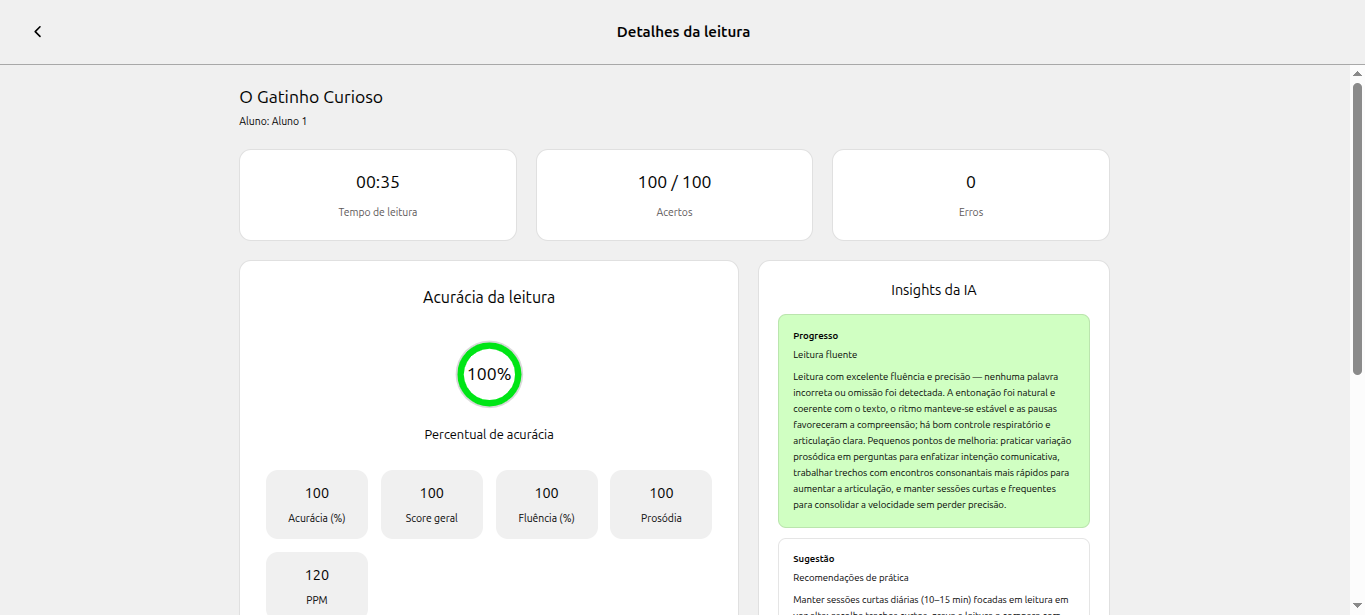
\includegraphics[width=0.8\textwidth]{sistema_2.png}
    \caption{Tela do Sistema YZW}
    \label{fig:etiqueta}
\end{figure}

\subsubsection{Fundamentação Arquitetural}

O sistema segue o padrão de Arquitetura em Camadas (\textit{Layered Architecture}). Nesse modelo, o software é organizado em níveis hierárquicos com dependências unidirecionais e contratos bem definidos entre interfaces. Essa organização favorece manutenibilidade, testabilidade e reutilização, e alterações internas de um componente pouco afetam as outras camadas quando os contratos são preservados.

Esse padrão foi preferido a arquiteturas baseadas em microserviços. Embora ofereçam elevada escalabilidade e independência de implantação, microserviços trazem complexidade operacional, necessidade de orquestração distribuída e custos de observabilidade que podem representar sobrecarga desnecessária em sistemas educacionais em estágio inicial de evolução~\cite{richards2020fundamentals}.

O backend do Sistema YZW é implementado em FastAPI, e essa organização resulta nas seguintes camadas funcionais:

\begin{table}[ht]
\centering
\footnotesize
\caption{Camadas arquiteturais do backend do Sistema YZW}
\label{tab:camadas-arquitetura}
\begin{tabular}{p{4cm} p{8cm}}
\toprule
\textbf{Camada} & \textbf{Responsabilidade} \\
\midrule
Apresentação &
Exposição de interfaces e validação de entradas por meio de \textit{schemas} tipados. \\

Lógica de Negócio &
Implementação das regras pedagógicas e orquestração dos serviços de IA. \\

Acesso a Dados &
Isolamento da persistência por meio de abstrações de repositório. \\

Dados &
Definição de entidades e mapeamento objeto-relacional. \\
\bottomrule
\end{tabular}
\end{table}

Essa estrutura mantém independentes a representação de dados, a lógica pedagógica e a infraestrutura computacional, o que permite evoluir o sistema de forma incremental sem comprometer sua integridade funcional.

\subsubsection{Correspondência entre Arquitetura Pedagógica e Arquitetura de Software}

A arquitetura pedagógica do sistema tem quatro componentes conceituais interdependentes: ambiente de tarefas, módulo de conhecimento do domínio, modelo do aluno e módulo pedagógico.

O ambiente de tarefas corresponde à camada de apresentação, responsável pela interação com o usuário e pela validação de dados. O módulo de conhecimento do domínio e o módulo pedagógico são implementados na camada de serviços, onde são executadas as regras de avaliação e inferência pedagógica. O modelo do aluno é representado na camada de persistência, que armazena o histórico longitudinal de desempenho e as interações educacionais.

Essa correspondência alinha objetivos pedagógicos e processos computacionais e reduz o risco de dissociação entre métricas técnicas e interpretação educacional.

\subsubsection{Arquitetura de Processamento e Pipeline Assíncrono}

O fluxo operacional do Sistema YZW é um \textit{pipeline} assíncrono orientado a eventos, baseado em um modelo de execução \textit{Async-First}. Essa abordagem desacopla as etapas de processamento, dá controle explícito sobre a exposição de dados sensíveis e permite escalar sob as cargas concorrentes típicas de ambientes educacionais digitais~\cite{kleppmann2017designing}.

A Figura~\ref{fig:arquitetura} reúne a estrutura em camadas do backend, o processamento biométrico local, o mecanismo de inferência pedagógica assistida por IA e o fluxo de disponibilização analítica para apoio à decisão educacional. Aquisição de dados, processamento acústico, extração de métricas, persistência estruturada e geração de diagnóstico pedagógico ficam separados, com contratos de comunicação entre os componentes.

\begin{figure}[ht]
    \centering
    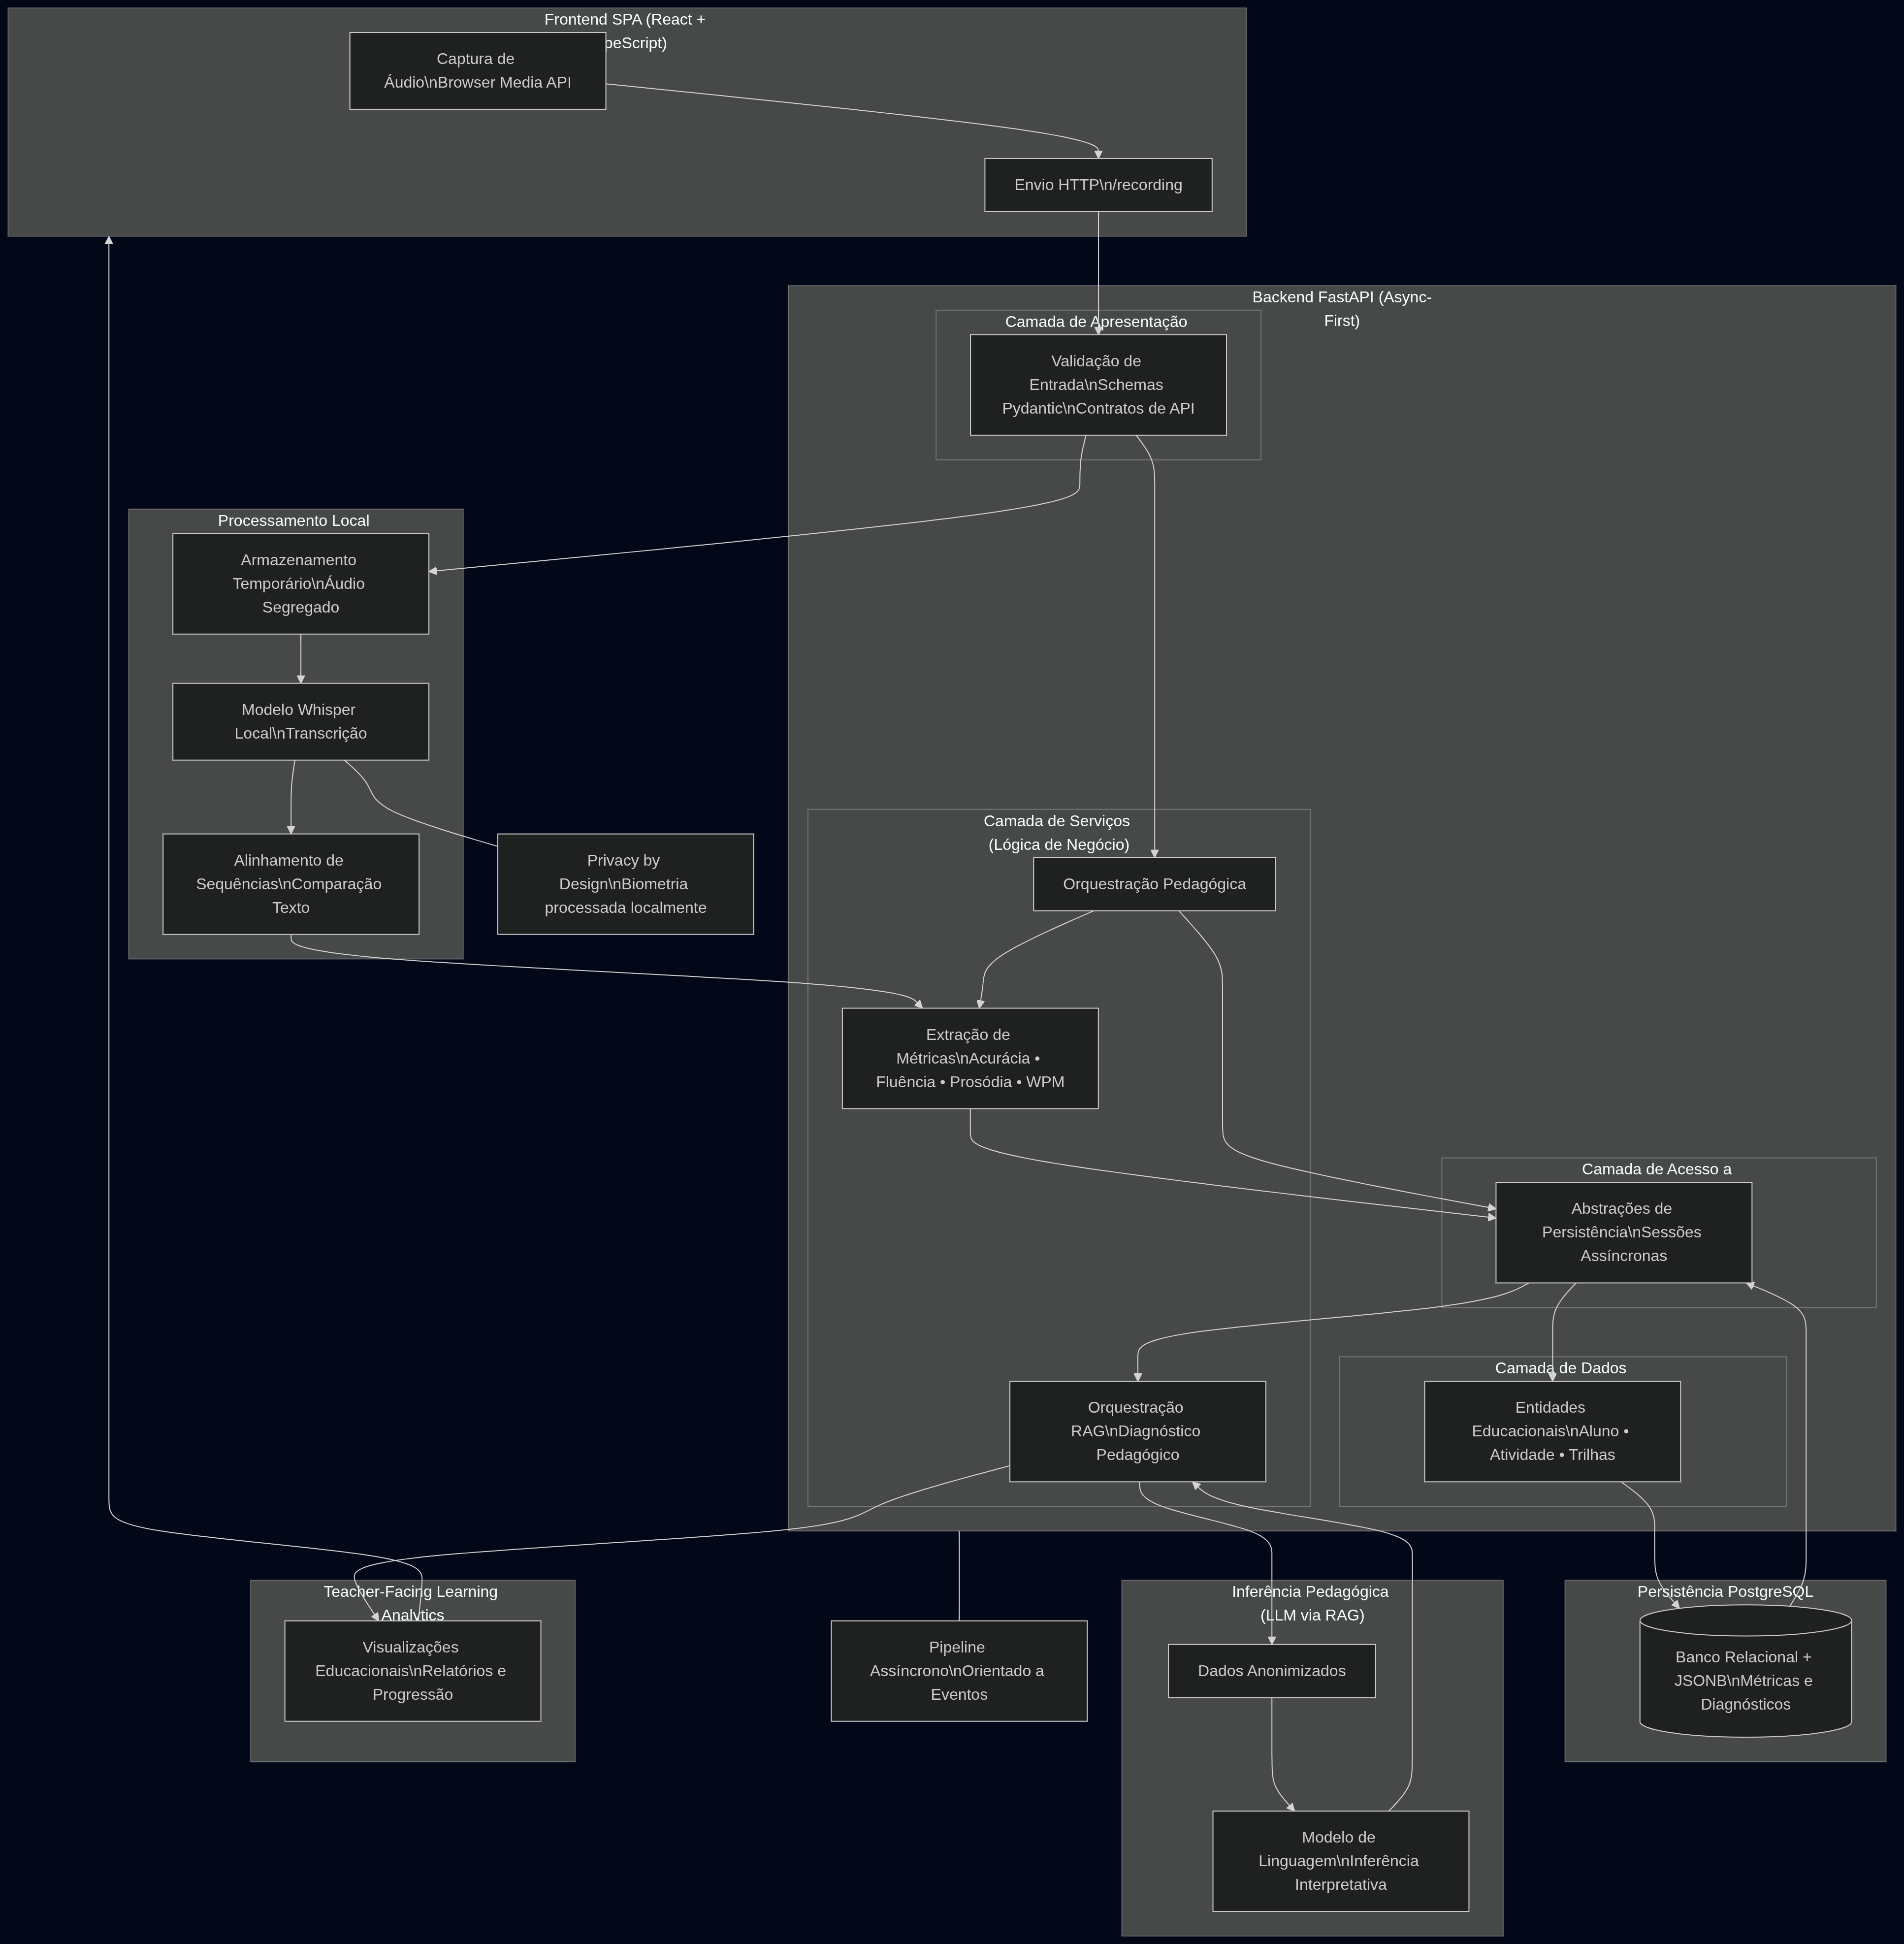
\includegraphics[width=0.85\textwidth]{esquema_arquitetura.png}
    \caption{Arquitetura integrada do Sistema YZW}
    \label{fig:arquitetura}
\end{figure}

O \textit{pipeline} é composto por estágios sequenciais com responsabilidades definidas e contratos de dados explícitos entre camadas, descritos a seguir.

\subsubsection{Aquisição e Ingestão de Dados}

A interface do usuário, uma aplicação de página única em React e TypeScript, captura o áudio da leitura por meio de APIs de mídia do navegador e o transmite ao backend por HTTP. A validação inicial, feita com \textit{schemas} Pydantic, verifica a conformidade com os contratos de entrada e evita que inconsistências se propaguem pelo \textit{pipeline}.

\subsubsection{Processamento Local e Transcrição}

O áudio é mantido em armazenamento temporário segregado e transcrito por um modelo Whisper~\cite{radford2023whisper} executado localmente. A execução local segue o princípio de \textit{Privacy by Design}, que preconiza incorporar a proteção de dados desde a concepção arquitetural do sistema~\cite{cavoukian2011privacy}. O resultado é uma representação textual normalizada acompanhada de metadados temporais.

\subsubsection{Extração de Métricas de Leitura}

Algoritmos de alinhamento de sequências comparam a transcrição da leitura com o texto de referência. Técnicas de reconhecimento automático de fala e análise de leitura têm sido amplamente utilizadas para avaliação educacional e mensuração de fluência e precisão. O sistema produz métricas estruturadas de acurácia textual, fluência temporal, prosódia e velocidade de leitura (palavras por minuto), coerentes com abordagens de avaliação automatizada de leitura baseadas em evidências acústicas e temporais.
% TODO(autores): definir cada métrica (fórmula de acurácia, como fluência e prosódia são calculadas, PPM) e que tipos de texto de referência o sistema aceita (pedido do revisor 2).

\subsubsection{Persistência e Governança de Dados}

Métricas e diagnósticos são armazenados em um banco relacional PostgreSQL, com campos JSONB. Antes da persistência, o sistema minimiza os dados e dissocia identificadores sensíveis. O procedimento segue princípios de governança e proteção de dados em sistemas digitais educacionais e reduz os riscos de reidentificação e de exposição indevida de informações pessoais~\cite{cavoukian2011privacy}. No Brasil, a Lei Geral de Proteção de Dados classifica o dado biométrico como dado pessoal sensível e dedica o art.~14 ao tratamento de dados de crianças e adolescentes~\cite{brasil2018lgpd}.

\subsection{Inferência Pedagógica Assistida por IA}

O diagnóstico pedagógico é gerado por \textit{Retrieval-Augmented Generation (RAG)}~\cite{lewis2020rag}, abordagem que combina recuperação de informações estruturadas com modelos de linguagem para produzir inferências contextualizadas. O sistema recupera o histórico longitudinal do estudante, constrói um contexto estruturado e submete essa representação padronizada a um modelo de linguagem.
% TODO(autores): informar qual LLM foi usado (modelo, versão, provedor) e o que é recuperado no RAG (pedido dos revisores 1 e 2).

A separação entre processamento biométrico local e inferência semântica remota forma uma arquitetura híbrida com governança explícita de privacidade, alinhada a práticas contemporâneas de sistemas de IA responsáveis~\cite{kleppmann2017designing}.

\subsection{Disponibilização Analítica}

Os resultados são enviados ao frontend e convertidos em visualizações interpretáveis. Nessa etapa o sistema funciona como uma plataforma de \textit{Learning Analytics} voltada ao professor, que liga o processamento automatizado à tomada de decisão pedagógica baseada em dados~\cite{siemens2012learning}.

A arquitetura suporta escalabilidade horizontal e desacoplamento entre etapas de processamento. A separação entre processamento sensível e inferência semântica também facilita a auditoria de decisões automatizadas e a governança de dados educacionais.

\subsection{Teste de usabilidade}
A plataforma foi avaliada por meio de um questionário baseado na Escala de Usabilidade de Sistema (SUS, \textit{System Usability Scale})~\cite{brooke1996sus}, composto por afirmações positivas e negativas intercaladas, medidas em uma escala Likert de 1 (discordo totalmente) a 5 (concordo totalmente). As afirmações aplicadas aos participantes estão na Tabela~\ref{tab:perguntas_sus_aplicadas}.

\begin{table}[ht]
\centering
\footnotesize
\caption{Afirmações de usabilidade aplicadas no questionário (Baseado na Escala SUS)}
\label{tab:perguntas_sus_aplicadas}
\begin{tabular}{c p{12cm}}
\toprule
\textbf{Questão} & \textbf{Afirmação Avaliada (Escala Likert 1 a 5)} \\
\midrule
1 & Eu acho que gostaria de usar este aplicativo com frequência. \\
2 & Eu acho que o aplicativo é excessivamente complexo. \\
3 & Eu precisaria de ajuda de uma pessoa com conhecimentos técnicos para usar o aplicativo. \\
4 & As diversas funções do aplicativo estão bem integradas. \\
5 & O sistema apresenta inconsistências durante a utilização. \\
6 & Imagino que as pessoas aprenderiam a usar este aplicativo rapidamente. \\
7 & Achei o aplicativo atrapalhado ou confuso de usar. \\
8 & Senti-me confiante ao utilizar o aplicativo. \\
9 & Precisei aprender várias coisas novas antes de conseguir usar o aplicativo. \\
\bottomrule
\end{tabular}
\end{table}

%Para isso, o estudo foi estruturado em trˆes etapas: i) definic¸ ˜ao dos testes de usabilidade (6.2.1); ii) selec¸ ˜ao dos participantes (6.2.2); e iii) coleta e an´alise dos resultados (6.2.3). Essas etapas orientam a metodologia adotada na avaliac¸ ˜ao da ferramenta

\section{Resultados e discussões}
\label{sec:resultado}
%A avaliação da plataforma foi conduzida por meio de um questionário baseado na Escala de Usabilidade de Sistema (SUS -- \textit{System Usability Scale}), composto por afirmações positivas e negativas intercaladas, mensuradas em uma escala Likert de 1 (discordo totalmente) a 5 (concordo totalmente).
O instrumento SUS permitiu examinar a percepção de facilidade de uso, integração funcional, confiança na utilização e possíveis barreiras de aprendizagem do \textit{Sistema YZW}. %As afirmações aplicadas aos participantes estão apresentadas na Tabela~\ref{tab:perguntas_sus_aplicadas}.


% TODO(autores): esclarecer o protocolo: os 9 avaliadores usaram o sistema com gravações de quem? Houve leituras de crianças (quantas, de onde, com que perfil)? Informar aprovação/dispensa do comitê de ética (pedido do revisor 2).
% TODO(autores): apresentar os dados do SUS (média por item e/ou escore), em tabela (pedido do revisor 3).
O painel de avaliadores ($n=9$) foi multidisciplinar e alinhado ao contexto de aplicação do sistema. Predominaram especialistas em Tecnologia, acompanhados de profissionais das áreas de Psicologia, Educação e Ciências Sociais. A maioria possui pós-graduação em nível de mestrado ou doutorado; cinco participantes têm mais de 10 anos de experiência, dois têm entre 5 e 10 anos e dois têm menos de 3 anos (incluindo o único participante com graduação em andamento).

A percepção de usabilidade foi amplamente positiva. As afirmações positivas tiveram médias elevadas, concentradas entre as pontuações 4 e 5. A maioria dos participantes declarou forte intenção de uso recorrente e alto nível de confiança durante a interação com o sistema. A percepção de aprendizado rápido foi praticamente unânime, o que sugere que a estrutura funcional e a organização das tarefas favorecem a compreensão operacional já no primeiro contato. A integração entre as funcionalidades também foi bem avaliada.

As afirmações negativas confirmam esse resultado. Na escala SUS, pontuações baixas nesses itens indicam melhor desempenho do artefato. As respostas rejeitaram de forma consistente a ideia de que o sistema seja confuso, inconsistente ou difícil de utilizar. A afirmação sobre o caráter ``atrapalhado'' da interface recebeu apenas notas 1 e 2, e a percepção de inconsistência também foi baixa.

A análise por perfil de usuário revelou um ponto de atenção. Um participante com mestrado em Psicologia e extensa experiência profissional ($>10$ anos) apresentou elevada intenção de uso e confiança na aplicação, mas atribuiu pontuação máxima (5) às afirmações sobre complexidade percebida, necessidade de suporte técnico e esforço de aprendizagem inicial. Esse resultado sugere que a experiência de uso varia conforme o repertório tecnológico prévio do usuário e que profissionais de áreas clínicas e educacionais (não tecnológicas) podem precisar de mais suporte inicial para alcançar autonomia na plataforma.

Os resultados preliminares indicam que o Sistema YZW foi bem aceito por usuários com diferentes níveis de experiência, que avaliaram positivamente a organização das informações e a disposição das ferramentas. As barreiras iniciais encontradas por perfis não técnicos indicam a necessidade de apoio complementar ao usuário. Para as próximas iterações, recomenda-se implementar tutoriais de introdução (\textit{onboarding}), simplificar terminologias e oferecer mecanismos de orientação contextual. O número de participantes é limitado para generalizações estatísticas, mas os dados são consistentes com os objetivos de uma avaliação inicial.
\section{Limitações e Trabalhos Futuros}
\label{sec:proximos-passos}

A prova de conceito demonstrou viabilidade técnica para automatizar etapas centrais da avaliação de fluência leitora. Para sustentar uso contínuo em ambientes escolares, com maior volume de usuários, diversidade de perfis e requisitos de governança, o Sistema YZW ainda demanda avanços arquiteturais e funcionais.

\subsection{Aprimoramento da Usabilidade e Acessibilidade}
A avaliação com a SUS mostrou que, apesar da aceitação amplamente positiva, profissionais de áreas clínicas e educacionais (como o perfil de Psicologia) enfrentam barreiras iniciais por terem menor familiaridade tecnológica. Para as próximas iterações de design estão previstos tutoriais de introdução (\textit{onboarding}), a simplificação de terminologias na interface e mecanismos de orientação contextual integrados às ferramentas do painel.

\subsection{Ampliação multimodal: análise de escrita e caligrafia}
Além da leitura oral, pretende-se incorporar a análise da escrita das crianças, para complementar o diagnóstico educacional com indicadores de grafomotricidade e precisão ortográfica. Como extensão do Sistema YZW, propõe-se um módulo de aquisição e processamento de escrita manuscrita, seguido da extração de métricas como legibilidade, regularidade do traçado, espaçamento entre letras e palavras, alinhamento em linha base, tamanho relativo de caracteres, consistência de inclinação e sinais indiretos de hesitação e correções.

Essas métricas podem ser integradas ao mesmo modelo de histórico do estudante e ao mecanismo de inferência pedagógica (RAG + LLM), unindo evidências de leitura e escrita em uma visão mais abrangente do processo de alfabetização.

\subsection{Geração de Planos Educacionais Individualizados (PEI)}

A geração de Planos Educacionais Individualizados (PEI) é uma extensão do sistema voltada a alunos com dificuldades de aprendizagem ou condições do neurodesenvolvimento, como Transtorno do Espectro Autista (TEA), TDAH e dislexia. A construção desses planos segue as diretrizes do Parecer CNE/CP nº 50/2023, que recomenda práticas educacionais inclusivas, baseadas em evidências, e o uso de instrumentos diagnósticos qualificados para atender às necessidades específicas de cada aluno~\cite{cne2023parecer50}.
Esse passo permitirá personalizar o ensino e melhorar a articulação entre escola, família e profissionais de saúde, como fonoaudiólogos e neuropediatras.

\section{Considerações Finais}
\label{sec:consideracoes}

A arquitetura híbrida protege dados biométricos sensíveis por meio do processamento local de voz (\textit{Privacy by Design}), enquanto o uso de LLMs via RAG permite inferências educacionais de alto nível. A avaliação SUS indicou boa usabilidade da interface e mostrou que a eficácia da ferramenta depende de tutoriais de \textit{onboarding} que ajudem profissionais das áreas clínicas e pedagógicas a superar barreiras tecnológicas.

O Sistema YZW estabelece uma base para a avaliação automatizada da alfabetização. Com os próximos passos, o sistema deve passar de instrumento de triagem a plataforma que articula escola, família e profissionais de saúde em intervenções preventivas, inclusivas e baseadas em evidências.

\bibliographystyle{sbc}
\bibliography{sbc-template}

\end{document}
